\documentclass[11pt,a4paper]{article}

%\usepackage{pdfsync} %% for pdfview (good PDF viewer for the Mac)
%\usepackage[active]{srcltx} %% for xdvi

\usepackage{verbatim}
\usepackage{graphicx}
\usepackage{parskip}
%\usepackage{epsfig}
\usepackage{url}
\usepackage[colorlinks=true]{hyperref}
\usepackage{listings}
\usepackage{color}

\usepackage{geometry}
\geometry{textwidth=38em,textheight=44\baselineskip}

\newcommand{\mycomment}[3]{{\ignorespaces\sffamily[~#1~(#2): #3~]}}
\renewcommand{\mycomment}[3]{\ignorespaces\relax}

\definecolor{Brown}{cmyk}{0,0.81,1,0.60}
\definecolor{OliveGreen}{cmyk}{0.64,0,0.95,0.40}
\definecolor{CadetBlue}{cmyk}{0.82,0.77,0.13,.4}
\definecolor{lightlightgray}{gray}{0.9}

\lstset{
%language=Java,                             % Code langugage
basicstyle=\ttfamily \small,                   % Code font, Examples: \footnotesize, \ttfamily
keywordstyle=\color{CadetBlue},        % Keywords font ('*' = uppercase)
commentstyle=\color{OliveGreen},              % Comments font
numbers=left,                           % Line nums position
%numberstyle=\tiny,                      % Line-numbers fonts
%stepnumber=1,                           % Step between two line-numbers
numbersep=5pt,                          % How far are line-numbers from code
%backgroundcolor=\color{lightlightgray}, % Choose background color
%frame=none,                             % A frame around the code
tabsize=4,                              % Default tab size
%captionpos=b,                           % Caption-position = bottom
%breaklines=true,                        % Automatic line breaking?
%breakatwhitespace=false,                % Automatic breaks only at whitespace?
showspaces=false,                       % Dont make spaces visible
showtabs=false,                         % Dont make tabls visible
showstringspaces=false,
%columns=flexible,                       % Column format
morecomment=[l]{//},
morekeywords={domain, types, bool, int, real, default, state, action, interm, observ, fluent, requirements, reward, deterministic, continuous, multivalued, intermediate, nodes, constrained, partially, observed, concurrent, integer, valued, pvariables, cpfs, cdfs, if, then, else, Bernoulli, Normal, KronDelta, Discrete, reward, instance, init, state, true, false, max, nondef, actions, horizon, discount, objects, non, fluents, constraints}
}

%\COMMENT begins comment
\long\def\COMMENT#1\ENDCOMMENT{\message{(Commented text...)}\par}

%% Check if pdflatex is running
\ifx\pdfoutput\undefined\def\pdfoutput{0}\fi

% Good KR language is notationally efficacious

%\bibliographystyle{alpha}
\pagestyle{empty}
\begin{document}
\title{\bf Relational Dynamic Influence Diagram Language (RDDL):
Language Description}
\author{
 \href{http://users.cecs.anu.edu.au/~ssanner/}{Scott Sanner} (\texttt{ssanner@gmail.com}) \\
NICTA and the Australian National University
}
\date{}

\maketitle

\vspace{-5mm}

\begin{abstract}
The Relational Dynamic Influence Diagram Language (RDDL) is a uniform
language where states, actions, and observations (whether discrete or
continuous) are parameterized variables and the
evolution of a fully or partially observed (stochastic) process is
specified via (stochastic) functions over next state variables
conditioned on current state and action variables (n.b.,
concurrency is allowed).  Parameterized variables are simply templates
for ground variables that can be obtained when given a particular
problem instance defining possible domain objects.  Semantically, RDDL
is simply a dynamic Bayes net (DBN)~\cite{dbn} (with potentially many
intermediate layers) extended with a simple influence diagram
(ID)~\cite{influence_diagrams} utility node representing immediate
reward.  An objective function specifies how these immediate rewards
should be optimized over time for optimal control.  For a ground
instance, RDDL is just a factored MDP (or POMDP, if partially
observed).
\end{abstract}

\vspace{-3mm}

\setcounter{tocdepth}{2}
\tableofcontents

\newpage
%\vfill

\section{What's wrong with (P)PDDL?}

In short, nothing is wrong with (P)PDDL.  Every planning domain
language serves a purpose to compactly specify a set of
planning problems with common characteristics for exploitation
by domain-independent (but domain language-specific) planners.

However, it would be unreasonable to assume there is one single
compact and correct syntax for specifying all useful planning
problems.  Thus, RDDL is not intended as a replacement for the PDDL family
of languages~\cite{pddl_family} or PPDDL~\cite{ppddl}, rather it is intended
to model a class of problems that are difficult to model with PPDDL
and PDDL.  If (P)PDDL suffices for a problem description, then
RDDL's expressivity is not needed.

As a motivating example for RDDL, we discuss the \emph{cell transition
model} (CTM) of traffic flow~\cite{ctm}, which requires the following
constructs not jointly expressible in (P)PDDL:
\begin{enumerate}
\item Each traffic signal is independently controlled by a concurrently executed action.
\item Cars move independently and stochastically.\footnote{While a careful
encoding of a \emph{probabilistic} effect under a \emph{forall} effect
can encode this in PPDDL, it is not clear there is any way to resolve
conflicting stochastic effects (two cars that stochastically move into
a traffic cell, where there is only room for one of them).}
\item The full CTM uses integers to model counts of vehicles,
real values to model traffic speed and density, and stochastic
difference equations to specify transitions.
\item The CTM dynamics are simple, complexity derives
from a nonfluent network topology.  One would like to plan
for \emph{given} nonfluents \emph{independent} of an initial state.
\item One would like to minimize traffic density in a CTM, which requires
\emph{summing} over \emph{all} traffic cells (which change with each domain instance).
\item In concurrent domains, action preconditions cannot be checked
locally, they must be checked globally, e.g., a joint configuration of
two or more traffic signals may be illegal.  For this one needs global
state-action constraint checks.
%state/action constraints for (a) action preconditions, 
%(b) as runtime assertions, and (c) for offline planners
%that cannot exploit initial state reachability.
\end{enumerate}

Many other domains are difficult to formalize in PPDDL.
Multi-elevator control with independent random arrivals, logistics
domains with independently moving vehicles and noise, and UAVs with
sensors for partially observed state are all important domains that
cannot be specified in PPDDL.  The obvious solution might simply be to
extend PPDDL, as PDDL has been extended numerous
times~\cite{pddl_family}.  However, stochastic effects and concurrency
are difficult to jointly reconcile in an effects-based language.  If we
take the approach that concurrent actions that possibly conflict
(c.f., \emph{probabilistic mutex}~\cite{pgraphplan}) are disallowed
--- similar to the way concurrency is handled in PDDL
2.1~\cite{pddl21} --- then we end up with a restrictive definition of
concurrency that prevents concurrent actions that may only conflict
1\% of the time.  Instead we opt for \emph{unrestricted
concurrency}~\cite{paragraph}, for which it appears there is no 
well-defined PDDL-style transition semantics.  Rather than add a layer of
stochastic conflict resolution to PPDDL, a dynamic Bayes net
(DBN)~\cite{dbn} transition formalism offers a simple solution --- hence
the motivation for RDDL.

\section{Principles of RDDL}

RDDL is influenced by the PDDL family~\cite{pddl_family},
PPDDL~\cite{ppddl}, stochastic programs~\cite{stochastic_programs},
influence diagrams~\cite{influence_diagrams}, the SPUDD~\cite{spudd}
and Symbolic Perseus~\cite{pascal_thesis,sym_perseus_code}
representations for factored MDPs and POMDPs, first-order probabilitic
inference (FOPI) -- especially \emph{parfactors}~\cite{fopi03}, and (factored)
first-order MDPs and POMDPs~\cite{fomdp,ffomdp,fo_pomdp}.  

A central design principle of RDDL is that the language should be
simple and uniform with its expressive power deriving from
composition of simple constructs.

\subsection{What RDDL Is}

RDDL is based on the following principles:

\begin{itemize}
\item \emph{Everything} is a a parameterized variable (fluent or nonfluent)
  \begin{itemize}
    \item Action fluents 
    \item State fluents 
    \item $[$Optional$]$ Observation fluents (for partially observed domains)
    \item $[$Optional$]$ Intermediate fluents (derived predicates, correlated effects, \ldots)
    \item $[$Optional$]$ Constant nonfluents (general constants, topology relations, \ldots)
  \end{itemize}
\item Flexible fluent types
  \begin{itemize}
    \item Binary (predicate) fluents
    \item Multi-valued (enumerated) fluents
    \item Integer and continuous fluents (numerical fluents from PDDL 2.1~\cite{pddl21})
  \end{itemize}
\item The semantics is simply a \emph{ground Dynamic Bayes Net (DBN)}
  \begin{itemize}
    \item Supports factored state and observations
    \item Supports factored actions, hence concurrency (and never conflicts!)
    \item Supports intermediate state fluents for multi-layered DBNs
       \begin{itemize}
          \item Express (stochastic) derived predicates (c.f., PDDL 1.2~\cite{pddl12} and 2.2~\cite{pddl22})
          \item Express correlated effects
          \item Stratification by levels enforces a well-defined relational multi-layer DBN
       \end{itemize}
    \item Naturally supports independent exogenous events
  \end{itemize}
\item General expressions in transition and reward functions
  \begin{itemize}
    \item Logical expressions ($\land,|,\sim,=>,<=>$ plus $\exists$/$\forall$ quantification over variables)
    \item Arithmetic expressions ($+,-,*,/$ plus $\sum$/$\prod$ aggregation over variables)
    \item (In)equality comparison expressions ($==, \sim=, <, >, <=, >=$)
    \item Conditional expressions (if-then-else, switch)
    \item Basic probability distributions (Bernoulli, Discrete, Normal, Poisson, ...)
  \end{itemize}
\item Classical Planning as well as General (PO)MDP objectives
  \begin{itemize}
    \item Arbitrary reward (goals, numerical preferences) (c.f., PDDL 3.0~\cite{pddl3})
    \item Finite horizon
    \item Discounted or undiscounted
  \end{itemize}
\item State/action constraints% (from~\cite{pddl12})
  \begin{itemize}
    \item Encode legal actions (i.e., action preconditions)
    \item Assert state invariants (e.g., a package cannot be in two locations)
  \end{itemize}
\end{itemize}

\subsection{What RDDL Isn't (Yet)}

Notably, RDDL does not (at this time) support the following
language features:

\begin{itemize}
  \item Continuous time (c.f., PDDL2.1~\cite{pddl21})
  \item Durative actions / options / semi-(PO)MDPs (c.f., PDDL2.1~\cite{pddl21}, also \emph{options}~\cite{sutton_options})
  \item Temporal state/action goals or preferences (c.f., PDDL3.0~\cite{pddl3})
  \item Non-determinism or strict uncertainty  (c.f., \texttt{oneof} construct in PPDDL~\cite{ppddl})
  \item Game-theoretic constructs (c.f., Game Description Language (GDL)~\cite{gdl})
  \item Object fluents (c.f., PPDDL3.1/functional STRIPS~\cite{functional_strips}; enumerated types can substitute when the number of enumerated type values is fixed for all instances)
\end{itemize}

All features other than continuous time would be straightforward to add to 
RDDL. % and may be added in a future language revision (depending on demand).

\section{RDDL Examples}

Before we provide a formal language description, 
perhaps the best introduction to the language is through a
few examples.

\subsection{Simple Boolean Propositional Domain}

We begin with a simple use of RDDL to encode a non-parameterized
DBN with three boolean state variables $p,q,r$ and one boolean
action variable $a$.

%%%%%%%%%%%%%%%%%%%%%%%%%%%%%%%%%%%%%%%%%%%%%%%%%%%%%%%%%%%%%%
\newpage
\begin{lstlisting}[title=dbn\_prop.rddl]
////////////////////////////////////////////////////////////////////////
// A simple propositional 2-slice DBN (variables are not parameterized).
//
// Author: Scott Sanner (ssanner [at] gmail.com)
////////////////////////////////////////////////////////////////////////
domain prop_dbn {
  	
	requirements = { reward-deterministic };
      	
	// Define the state and action variables (not parameterized here)
	pvariables { 
		p : { state-fluent,  bool, default = false };
		q : { state-fluent,  bool, default = false };
		r : { state-fluent,  bool, default = false }; 
		a : { action-fluent, bool, default = false }; 
	};
  
	// Define the conditional probability function for each next
	// state variable in terms of previous state and action
	cpfs {
		p' = if (p ^ r) then Bernoulli(.9) else Bernoulli(.3);
						
		q' = if (q ^ r) then Bernoulli(.9) 
						else if (a) then Bernoulli(.3) else Bernoulli(.8);

		r' = if (~q) then KronDelta(r) else KronDelta(r <=> q);										
	};
    	
	// Define the reward function; note that boolean functions are 
	// treated as 0/1 integers in arithmetic expressions
	reward = p + q - r; 
}
        
// Define an instance of the above problem specifying an initial
// state and objective to achieve (discount and horizon)
instance inst_dbn {

	domain = prop_dbn;	
	init-state { 
		p = true;  // could also just say 'p' by itself 
		q = false; // default so unnecessary, could also say '~q' by itself
		r;         // same as r = true
	};
  
	max-nondef-actions = 1; // No concurrency here, so set to 1
	horizon  = 20;
	discount = 0.9;
}
\end{lstlisting}
%%%%%%%%%%%%%%%%%%%%%%%%%%%%%%%%%%%%%%%%%%%%%%%%%%%%%%%%%%%%%%

%%%%%%%%%%%%%%%%%%%%%%%%%%%%%%%%%%%%%%%%%%%%%%%%%%%%%%%%%%%%%%
\begin{figure}[t!]
\begin{center}
%angle=-90
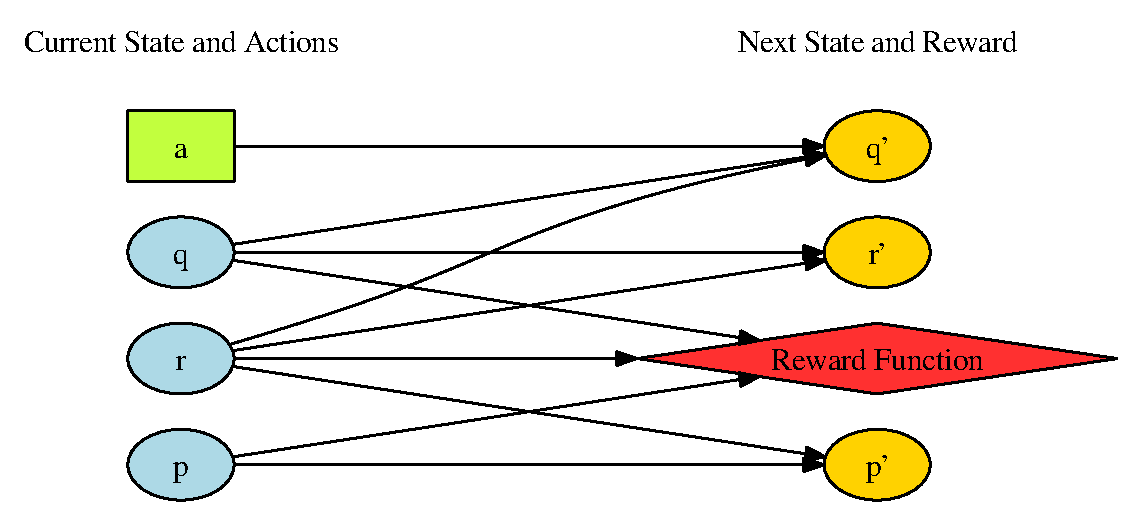
\includegraphics[scale=.6]{dbn_prop.pdf}
\caption{DBN and influence diagram 
for \texttt{dbn\_prop.rddl} automatically
produced by \texttt{rddl.viz.RDDL2Graph} in \texttt{rddlsim} Java 
package~\cite{rddlsim}.}
\label{fig:rddl1}
\end{center}
\end{figure}
%%%%%%%%%%%%%%%%%%%%%%%%%%%%%%%%%%%%%%%%%%%%%%%%%%%%%%%%%%%%%%

Before getting into details of this domain definition, we note
that it can be simply represented by a DBN~\cite{dbn} and 
influence diagram~\cite{influence_diagrams}
as provided in Figure~\ref{fig:rddl1}.

Following is a line-by-line discussion of the domain description:
\begin{itemize}  
\item All domains need an identifying name (here \texttt{prop\_dbn})
provided on line 6.
\item Domains should list their requirements as done on line 8, see
Section~\ref{sec:req} for a listing of possible requirements and their
meaning.
\item Lines 11--16 define parameterized variables (pvariables),
although in this case we do not use parameters so these
variables are in fact just the simple boolean propositional variables.  
\texttt{default} is used to specify the most common value of a pvariable, which
is useful for minimizing communication in client/server interaction.
\item Lines 20--27 list the domain transition function.  Next-state variables
are shown primed ($p',q',r'$) to differentiate them from current
state variables ($p,q,r$).  The definition
for $p'$ simply gives the following conditional probability $P(p'|p,r)$:
{\small \begin{equation}
  \begin{tabular}{|l|l|l||l|} 
  \hline
   $p$ & $r$ & $p'$ & $P(p'|p,q)$ \\ \hline \hline
   {\it true}  & {\it true}  & {\it true}  & 0.9 \\ \hline
   {\it true}  & {\it true}  & {\it false} & 0.1 \\ \hline
   {\it true}  & {\it false} & {\it true}  & 0.3 \\ \hline
   {\it true}  & {\it false} & {\it false} & 0.7 \\ \hline
   {\it false} & {\it true}  & {\it true}  & 0.3 \\ \hline
   {\it false} & {\it true}  & {\it false} & 0.7 \\ \hline
   {\it false} & {\it false} & {\it true}  & 0.3 \\ \hline
   {\it false} & {\it false} & {\it false} & 0.7 \\ \hline
  \end{tabular}
\end{equation}}
Likewise a similar conditional probability can be generated for
$P(q'|q,r,a)$; note here that the transition probability is dependent
upon the action $a$.  $P(r'|r,q)$
is a conditional expression over a Kronecker delta function.  A Kroneckor delta
simply places probability 1.0 on it's argument and 0 on all other
possible values, so it is useful whenever a transition is
deterministic.  Here, if $q$ is false, then $r'$ is assigned the value
of $r$, otherwise $r'$ is assigned the boolean value of the logical
expression $r \Leftrightarrow q$.  Note that if the argument of a
delta function is from a continuous domain rather than a discrete
domain, the Dirac delta function \texttt{DiracDelta} would be used
instead.
\item Line 31 lists the reward function, which determines what the
agent should optimize at each step of time.  Here we note that boolean
variables are used in an arithmetic expression; whenever a logical
expression is used in such an arithmetic expression, {\it true} is treated
as 1 and {\it false} as 0.
\item Lines 36--48 define an instance of this domain.  Typically an
instance will define domain objects, but this is not a parameterized
domain, so only an initial state, action restrictions, and objective
are provided here.
\begin{itemize}
\item \texttt{init-state} lists ground fluent atoms and their truth
assignment.  Default fluent assignments need not be provided, but it is
not an error to do so. 
\item \texttt{max-nondef-actions} is used to specify how
many actions in a domain are allowed to use a non-default value -- a
value larger than 1 would be specified for concurrent domains, but for
non-concurrent domains like this one, a value of 1 should be used.
\item The objective evaluated by RDDL is simply the expected (i.e.,
average) sum of discounted rewards over multiple trials, where here
the \texttt{discount} factor $\gamma = 0.9$ and \texttt{horizon}
$h=20$.  At the end of each trial, the RDDL simulator returns the
value $V_{\pi}(s_0)$ for the state-action trajectory encountered
during the trial starting from the \texttt{init-state} definition of
state $s_0$ and following the client agent's policy $\pi: S
\rightarrow A$ which provides an action $a \in A$ for each state $s
\in S$ encountered during the trial:
\begin{equation}
V_{\pi}(s_0) = \sum_{t=0}^{h} \gamma^t \cdot R(s_t,\pi(s_t)).
\end{equation}
Here $R(s_t,a_t)$ is the \texttt{reward} (sampled if requirement 
\texttt{reward-deterministic} is not specified)
in state $s_t$ at time $t$ when action $a_t = \pi(s_t)$ is taken.
The state trajectory $(s_0,\ldots,s_h)$ 
is simply sampled according to the defined
\texttt{cpfs}.
\end{itemize}
\end{itemize}

\subsection{Non-parameterized Partially-observed Domain}

Before we move on to a true relational parameterized domain example, we
first extend the previous \texttt{dbn\_prop.rddl} with defined
enumerated types, intermediate variables, and partial observability.

%%%%%%%%%%%%%%%%%%%%%%%%%%%%%%%%%%%%%%%%%%%%%%%%%%%%%%%%%%%%%%
\newpage
\begin{lstlisting}[title=dbn\_types\_interm\_po.rddl]
////////////////////////////////////////////////////////////////////////
// A simple DBN (variables are not parameterized) exhibiting use of
// bools, ints, reals, enumerated types, intermediate variables, and
// observation variables.
//
// Author: Scott Sanner (ssanner [at] gmail.com)
////////////////////////////////////////////////////////////////////////
domain prop_dbn2 {
  	
	requirements = { 
		reward-deterministic, // Reward is a deterministic function
		integer-valued,       // Uses integer variables
		continuous,           // Uses continuous variables
		multivalued,          // Uses enumerated variables
		intermediate-nodes,   // Uses intermediate nodes
		partially-observed    // Uses observation nodes 
	};
      	
	// User-defined types
	types {
		enum_level : {@low, @medium, @high}; // An enumerated type
	};

	pvariables { 
		p : { state-fluent,  bool, default = false };
		q : { state-fluent,  bool, default = false };
		r : { state-fluent,  bool, default = false };
		 
		i1 : { interm-fluent, int,        level = 1 };
		i2 : { interm-fluent, enum_level, level = 2 };
		
		o1 : { observ-fluent, bool };
		o2 : { observ-fluent, real };
		
		a : { action-fluent, bool, default = false }; 
	};
  
	cpfs {

		// Some standard Bernoulli conditional probability tables
		p' = if (p ^ r) then Bernoulli(.9) else Bernoulli(.3);
						
		q' = if (q ^ r) then Bernoulli(.9) 
						else if (a) then Bernoulli(.3) else Bernoulli(.8);

		// KronDelta is a delta function for a discrete argument
		r' = if (~q) then KronDelta(r) else KronDelta(r <=> q);
		
		// Just set i1 to a count of true state variables
		i1 = KronDelta(p + q + r); 
		
		// Choose a level with given probabilities that sum to 1
		i2 = Discrete(enum_level, 
						@low : if (i1 >= 2) then 0.5 else 0.2,
						@medium : if (i1 >= 2) then 0.2 else 0.5,
						@high : 0.3
					);							
		
		// Note: Bernoulli parameter must be in [0,1]
		o1 = Bernoulli( (p + q + r)/3.0 ); 

		// Conditional linear stochastic equation
		o2 = switch (i2) {
				case @low    : i1 + 1.0 + Normal(0.0, i1*i1),  
				case @medium : i1 + 2.0 + Normal(0.0, i1*i1/2.0), 
				case @high   : i1 + 3.0 + Normal(0.0, i1*i1/4.0) };
	};
    	
	// A boolean functions as a 0/1 integer when a numerical value is needed
	reward = p + q - r + 5*(i2 == @high); 
}
        
instance inst_dbn {
	domain = prop_dbn2;	
	init-state { p; r; };
	max-nondef-actions = 1;
	horizon  = 20;
	discount = 0.9;
}
\end{lstlisting}
%%%%%%%%%%%%%%%%%%%%%%%%%%%%%%%%%%%%%%%%%%%%%%%%%%%%%%%%%%%%%%

%%%%%%%%%%%%%%%%%%%%%%%%%%%%%%%%%%%%%%%%%%%%%%%%%%%%%%%%%%%%%%
\begin{figure}[t!]
%\begin{center}
%angle=-90
\hspace{-15mm} 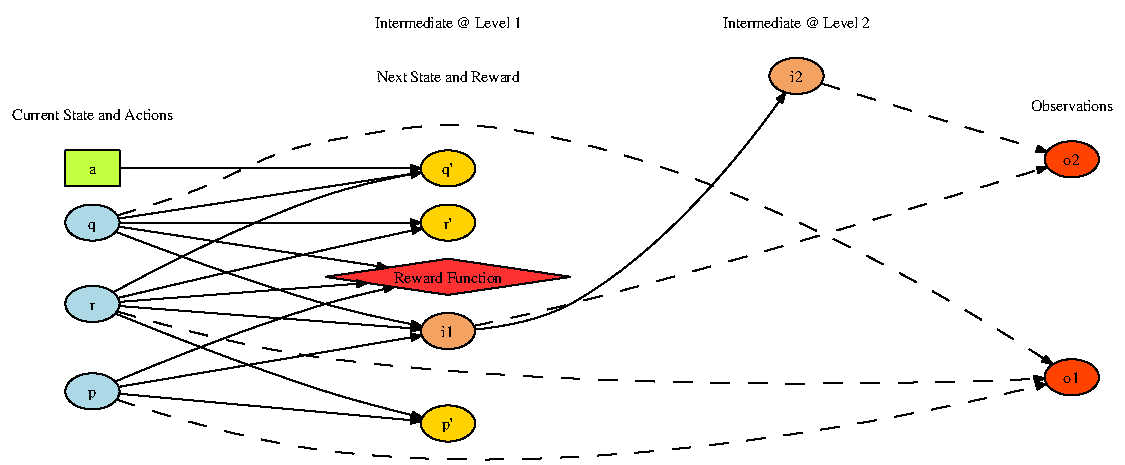
\includegraphics[scale=.9]{dbn_types_interm_po.pdf}
\caption{DBN and influence diagram 
for \texttt{dbn\_types\_interm\_po.rddl} automatically
produced by \texttt{rddl.viz.RDDL2Graph} in \texttt{rddlsim} Java 
package~\cite{rddlsim}.}
\label{fig:rddl2}
%\end{center}
\end{figure}
%%%%%%%%%%%%%%%%%%%%%%%%%%%%%%%%%%%%%%%%%%%%%%%%%%%%%%%%%%%%%%

The DBN and influence diagram for this RDDL description is provided in
Figure~\ref{fig:rddl2}.

Here we simply cover the differences between this domain and the
previous domain \texttt{dbn\_prop.rddl}.
\begin{itemize}  
\item In lines 10--17, we've added a number of requirements since
this domain uses integer, continuous, and multivalued (enumerated)
pvariables in addition to boolean variables.  The domain uses
intermediate variables that help determine the next state, but are
not part of the state.  
Also the domain is partially observed,
which means that in simulation, the server will determine both
state and observations during simulation, but only provide the
observations to the client agent for use in its policy decision.
\item Lines 20--22 define the possible values for a user-defined
enumerated (multivalue) type named \texttt{enum\_level}.
\item Lines 24--36 present additional pvariable definitions for
the intermediate and observation fluents.  Again, parameters are not used
here, but here we show types can also be \texttt{int}, \texttt{real},
or any of the user-defined types, in this case \texttt{enum\_level}.
Intermediate fluents must list a level of stratification. 
Intermediate variables are 
strictly stratified so that an intermediate variable can only
condition on intermediate pvariables of a strictly lower level,
or state pvariables.  Intermediate and observation pvariables do not
specify a default value.
\item Lines 40--47 start with cpf definitions that are identical 
to the previous domain.
\item Line 50 shows a simple cpf for an \texttt{int} type, where the
value of intermediate variable \texttt{i1} is simply deterministically
set to the sum $p + q + r$ (which takes values in $\{0,1,2,3\}$).  For
an actually stochastic distribution, a \texttt{Poisson} with an
appropriate rate parameter could be used in place of this
\texttt{KronDelta}.
\item Lines 53--57 show a useful way to sample a multivalued parameter
from a \texttt{Discrete} distribution (the $k$-ary extension of the
\texttt{Bernoulli} distribution).  The first parameter here specifies
the variable type being sampled (so that the simulator can perform
type-checking).  Next, each of the possible values are listed with the
probabilities of each value.  Note that these values must sum to 1.0
(otherwise the RDDL simulator will complain that the distribution is
not well-defined).  \texttt{i2} conditions on \texttt{i1} to determine
the distribution and one will note that it sums to 1.0 for all values
of \texttt{i1}.
\item Line 60 is a standard Bernoulli sample where we simply show here
that the parameters of any expression or random variable, can themselves
be expressions.  A Bernoulli parameter must be in $[0,1]$ and one can
verify this expression guarantees that property; such properties are
checked at runtime by the RDDL simulator.
\item Lines 63--66 show that RDDL can be easily used to encode
(stochastic) difference equations and via composition, more complex
constructs like the \emph{conditional} stochastic difference equation
shown here, which makes use of a \texttt{switch} statement over
various enumerated values of intermediate variable \texttt{i1}.
We point out here that the parameters of distributions, in this case
\texttt{Normal} with respective $\mu$ and $\sigma^2$ parameters, can
be expressions.
\item Line 70 demonstrates that intermediate pvariables can be used in a
reward, and also that logical equality \texttt{==} can be used with 
any pvariable.%, including enumerated types.
\end{itemize}
For a full listing of distributions that can be currently used with
RDDL, please see Section~\ref{sec:cpfs}.

\subsection{Parameterized Domain: Concurrent Interactive Game of Life}

Previously we showed non-parameterized RDDL domains that showed off
the expressiveness of the language for specifying factored MDPs and
POMDPs with potentially hybrid mixes of multivalued, integer, or
continuous states and actions.

Already, this non-parameterized version of RDDL makes for quite an 
expressive language, but it is not always compact when variables
and their cpfs must be repeated in a domain.

For example, a traffic domain can be modeled with traffic cells and
all cells have essentially the same behavior --- traffic flows into a
cell from upstream cells when a cell is not at full capacity, and
traffic flows out of a cell when the traffic signals permit and the
downstream cells are not at capacity.  There are simple rules that
govern the behavior of a traffic cell and hence it does not make sense
to repeatedly copy these rules for \texttt{cell-1}, \texttt{cell-2},
\ldots, \texttt{cell-n}.  Obviously, here we would want to
parameterize (i.e., lift) the transition dynamics and this 
requires parameterizing the RDDL DBN.

In Section~\ref{sec:other_domains}, we provide an external link to the
parameterized traffic domain specified in RDDL; however, because
traffic is a fairly complex domain, we instead choose to demonstrate
the parameterized DBN properties of RDDL in an interactive,
stochastic, and potentially concurrent version of John H. Conway's
\emph{Game of Life}~\cite{game_of_life}.

In short, the Game of Life specifies simple rules for a cellular
automata where the next state properties of a cell depend on its
surrounding cells.  In the following RDDL description, we parameterize
cells by their $(x,y)$ coordinates and specify neighboring cells
by a nonfluent boolean pvariable.  The cpf transition function
dynamics are based on the original rules plus some additional
enhancements for stochasticity, resetting a dead row, 
and agent interaction --- an agent can concurrently set a number
of cells up to \texttt{max-nondef-actions} defined in an instance.
We note that this domain explicitly defines the neighbor topology with
nonfluents, thus allowing a lifted planner to exploit a fixed
topology in its solution.

% Stochastic concurrent, update web

%%%%%%%%%%%%%%%%%%%%%%%%%%%%%%%%%%%%%%%%%%%%%%%%%%%%%%%%%%%%%%
\newpage
\begin{lstlisting}[title=game\_of\_life\_stoch.rddl]
////////////////////////////////////////////////////////////////////
// A simple DBN to encode Conway's cellular automata "game of life" 
// on a grid with some additional rules.  One gets a reward for 
// generating patterns that keep the most cells alive.
//
// Author: Scott Sanner (ssanner [at] gmail.com)
////////////////////////////////////////////////////////////////////
domain game_of_life {
  	
	requirements = { reward-deterministic };

	types { 
		x_pos : object;
		y_pos : object; 
	};
      	
	pvariables { 
		// Probability cell topology non-fluents (unchanging)
		PROB_REGENERATE : { non-fluent, real, default = 0.5 };
		NEIGHBOR(x_pos,y_pos,x_pos,y_pos) : {non-fluent,bool,default=false};
		
		// State, intermediate and action fluents
		alive(x_pos,y_pos) : { state-fluent, bool, default = false };
		count-neighbors(x_pos,y_pos) : { interm-fluent, int, level = 1 }; 
		set(x_pos,y_pos) : { action-fluent, bool, default = false };
	};
  
	cpfs {
		// Conway's game of life rules:
		// 1. Under-population: cell with < 2 live neighbors dies
   		// 2. Overcrowding:     cell with > 3 live neighbors dies
   		// 3. Survival:         cell with 2 or 3 live neighbors lives 
   		// 4. Reproduction:     cell with 3 live neighbors becomes live
   		//
   		// Scott's additional rules for RDDL:
   		// 5. Stochastic: above rules hold with PROB_REGENERATE certainty
   		// 6. Extra rule: all cells at same x-pos dead => random regeneration
   		// 7. Interactivity: agent can concurrently set different cells
		
		// Store alive-neighbor count for each cell
		count-neighbors(?x,?y) = 
		    KronDelta(sum_{?x2 : x_pos, ?y2 : y_pos} 
		              [NEIGHBOR(?x,?y,?x2,?y2) ^ alive(?x2,?y2)]);

		// Determine whether cell (?x,?y) is alive in next state
		alive'(?x,?y) = if (forall_{?y2 : y_pos} ~alive(?x,?y2))
							then Bernoulli(PROB_REGENERATE) // Rule 6

						else if ([alive(?x,?y)  
						          ^ (count-neighbors(?x,?y) >= 2)  
						          ^ (count-neighbors(?x,?y) <= 3)]
						         | [~alive(?x,?y) 
							       ^ (count-neighbors(?x,?y) == 3)]
						         | set(?x,?y))
						then Bernoulli(PROB_REGENERATE)
						else Bernoulli(1.0 - PROB_REGENERATE);
	};
    
    // Reward is number of alive cells
	reward = sum_{?x : x_pos, ?y : y_pos} alive(?x,?y);
	
	state-action-constraints {
		// Assertion: ensure PROB_REGENERATE is a valid probability
		(PROB_REGENERATE >= 0.0) ^ (PROB_REGENERATE <= 1.0); 
		
		// Precondition: perhaps we should not set a cell if already alive
		forall_{?x : x_pos, ?y : y_pos} alive(?x,?y) => ~set(?x,?y);
	};
}

// Define numerical and topological constants   
non-fluents game2x2 {
	domain = game_of_life;
	objects { 
		x_pos : {x1,x2};
		y_pos : {y1,y2};
	};
	non-fluents { 
		PROB_REGENERATE = 0.9; // Numerical constants are just non-fluents
		NEIGHBOR(x1,y1,x1,y2); NEIGHBOR(x1,y1,x2,y1); NEIGHBOR(x1,y1,x2,y2);
		NEIGHBOR(x1,y2,x1,y1); NEIGHBOR(x1,y2,x2,y1); NEIGHBOR(x1,y2,x2,y2);
		NEIGHBOR(x2,y1,x1,y1); NEIGHBOR(x2,y1,x1,y2); NEIGHBOR(x2,y1,x2,y2);
		NEIGHBOR(x2,y2,x1,y1); NEIGHBOR(x2,y2,x1,y2); NEIGHBOR(x2,y2,x2,y1);
	};
}
        
instance is1 {
	domain = game_of_life;	
	non-fluents = game2x2;
	init-state { 
		alive(x1,y1); 
		alive(x2,y2); 
	};
	max-nondef-actions = 3; // Allow up to 3 cells to be set concurrently
	horizon  = 20;
	discount = 0.9;
}
\end{lstlisting}
%%%%%%%%%%%%%%%%%%%%%%%%%%%%%%%%%%%%%%%%%%%%%%%%%%%%%%%%%%%%%%

%%%%%%%%%%%%%%%%%%%%%%%%%%%%%%%%%%%%%%%%%%%%%%%%%%%%%%%%%%%%%%
\begin{figure}[t!]
%\begin{center}
%angle=-90
\hspace{-5mm} 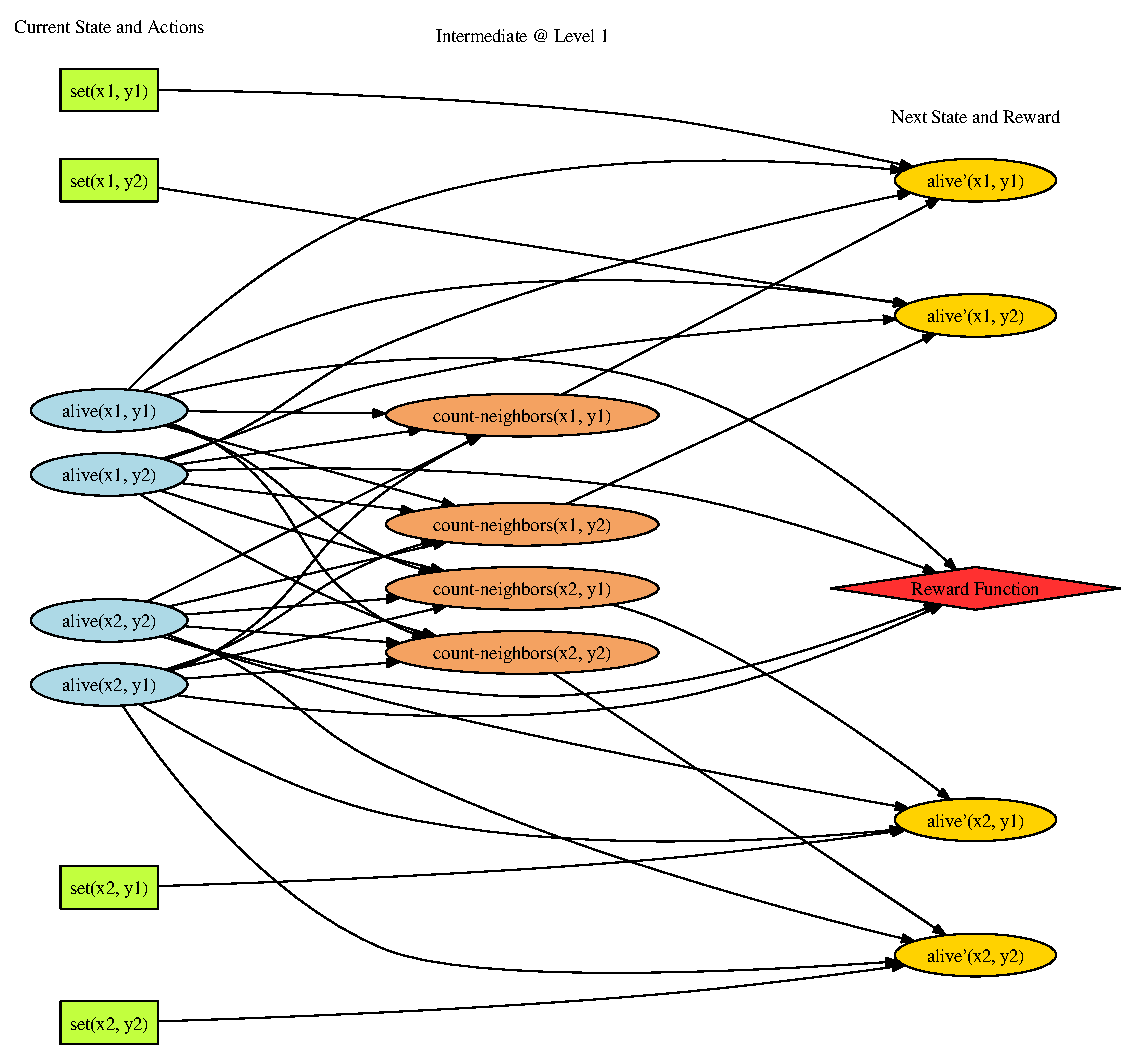
\includegraphics[scale=.81]{game_of_life2.pdf}
\caption{DBN and influence diagram 
for \texttt{game\_of\_life\_stoch.rddl} automatically
produced by \texttt{rddl.viz.RDDL2Graph} in \texttt{rddlsim} Java 
package~\cite{rddlsim}.}
\label{fig:rddl3}
%\end{center}
\end{figure}
%%%%%%%%%%%%%%%%%%%%%%%%%%%%%%%%%%%%%%%%%%%%%%%%%%%%%%%%%%%%%%

The DBN and influence diagram for this RDDL description and instance
\texttt{is1} is provided in Figure~\ref{fig:rddl3}.  This diagram is
crucial for understanding that the \emph{semantics of RDDL} is simply
\emph{a DBN over the ground pvariables of the domain instance}.

Perhaps the most {\bf confusing issue for those familiar with PPDDL}
will be the {\bf semantics of parameterized actions in RDDL}.  For
this we again refer to Figure~\ref{fig:rddl3} where we note that there
are \emph{four ground action fluents} denoted by green rectangles.  We
note that \emph{each} of these ground fluents is a \emph{separate
variable} taking on a distinct value determined by the user, and if we
examine line 54 of the cpf for \texttt{alive}, we see that it
conditions on \emph{all} of these ground action fluent truth value 
assignments as needed.

This is in contrast to the PPDDL view of actions where all of the
action information is given in the action name and parameters.  Here
an action is not viewed as a parameterized variable so it
does not make sense to say a PPDDL action consists of multiple
ground boolean variables (or
int, real, or enumerated variables) as is the case in RDDL.

The view of RDDL actions as templates for ground variables directly
supports concurrency.  If actions are boolean pvariables as for the
action pvariable \texttt{alive} in the Game of Life domain and {\it
false} is the default value, then taking a single action in domain
instance \texttt{is1} corresponds to setting any one of
$\mathit{set}(x1,y1), \mathit{set}(x1,y2), \mathit{set}(x2,y1),
\mathit{set}(x2,y2)$ to be true and the rest to be false.  This
corresponds to the non-concurrent case where
\texttt{max-nondef-actions=1} and only one action is executed at time.
However, if \texttt{max-nondef-actions=3} then up to three of
$\mathit{set}(x1,y1), \mathit{set}(x1,y2), \mathit{set}(x2,y1),
\mathit{set}(x2,y2)$ can be set to true, thereby allowing up to three
concurrent actions.  One will note that the cpf semantics for
\texttt{alive} in the Game of Life domain description still holds in
this concurrent case; hence, changing \texttt{max-nondef-actions} is
all that is needed to control concurrency in RDDL.\footnote{Of course,
if multiple concurrent actions could interfere with each other, this
would have to be handled directly in the cpf semantics for any
affected pvariables.  This is addressed in the Sidewalk domain
referenced in Section~\ref{sec:other_domains}.}

Having explained some of the major details of
\texttt{game\_of\_life\_stoch.rddl}, we proceed to highlight some
remaining novel aspects of this domain:
\begin{itemize}  
\item In lines 12--15, we've defined two user-defined object
types for the x and y positions used to parameterize
cells in the Game of Life.
\item In lines 17--26, we note the definition of pvariables
with parameters.  Here the parameters listed are just the
object types previously defined.
\item In lines 19--20, we first note the definition of non-fluent
pvariables.  This is used for any pvariables that will not change
during planning, but which can change between instances.
Non fluents can be specified separately from an instance
as shown in line 72 and referenced in the instance \texttt{is1}
on line 89.
\item In lines 29--57, we define parameterized cpfs:
\begin{itemize}
\item In lines 41--43, since the count of alive neighbors of a
cell is needed multiple times to determine the next state of
every cell, we simply compute it for each cell and store it
in a temporary intermediate variable.  We note here the use
of a \texttt{sum} over x and y position objects to perform
this sum over all possible neighboring cells.  As before,
logical expressions (here in $[\ldots]$) are treated as 0/1
values when used in an arithmetic expression (here \texttt{sum}).
\item Line 46 implements the rule to determine whether each cell is
alive in the next state.  Lines 46--47 use a universal quantifier over
objects in the \texttt{if} condition test to implement Rule 6 in the
comments, lines 49--54 implement Conway's standard rules, and lines
55--56 simply make the outcome predicted by Conway's rules stochastic
according to the non-fluent \texttt{PROB\_REGENERATE}.
\end{itemize}
\item Line 60 specifies the deterministic reward, which is simply
a sum over alive cells (again, this sum scales with the number
of cells in a particular domain instance).
\item Lines 62--68 demonstrate \texttt{state-action} constraints,
which have not been used previously.  \texttt{state-action} constraints
serve the following two purposes:
\begin{itemize}
\item \emph{Logical assertions} on all states that can be reached from
any legal initial state.  For example, line 64 ensures that the
\texttt{PROB\_REGENERATE} pvariable is a valid probability in $[0,1]$.
Such a constraint could also apply to any (quantified)
logical expression over fluents.
\item \emph{Action preconditions} for local and global precondition
checks.  Because preconditions in concurrent domains
must be checked globally --- two or more actions may mutually constain
each other --- we adopt the uniform approach of specifying
all action preconditions in the
\texttt{state-action} constraints section, whether concurrent or not.
An example of a simple \emph{local}
action precondition is given in line 67.
\end{itemize}
Any joint state and action that violate a \texttt{state-action}
constraint during a trial should cause the RDDL trial simulator
to abort in error since there was either an error in the domain
description leading to an illegal state, or the agent made an
error in the policy and tried to execute an illegal action.
\emph{Implicitly, if the agent only executes legal actions, then all
possible sampled trajectories should satisfy the state-action
constraints.}  State-action constraints are crucial for
lifted and regression-style planners that plan independently
of any initial state (and hence cannot exploit reachability
from an initial state to determine legal states).
\item Lines 72--85 define a non-fluents section where a cell topology
is specified.  This particular assignment to non-fluents is referenced
in line 89 of the instance definition.  The separation of non-fluents
from an initial state is intended to support lifted planning that is 
independent of an initial state, while allowing a planner to exploit
specific nonfluent structure common to many problem instances
(e.g. a cellular topology for the Game of Life, or a road network
in a logistics domain).
\item Line 94 specifies that \texttt{max-nondef-actions=3}, which
is used to allow multiple \texttt{set} actions to be executed
concurrently in this domain as explained previously.  If this
domain is intended to support only serial actions then 
this should be changed to \texttt{max-nondef-actions=1}.
\end{itemize}

\subsection{Additional Models}

\label{sec:other_domains}

RDDL is a very expressive language, so to give the reader a
sense of a few other interesting domains that can be encoded in
RDDL, we refer them to the following domains (with external links that
are hosted on the \texttt{rddlsim} code repository~\cite{rddlsim}):
\begin{itemize}
\item
\href{http://code.google.com/p/rddlsim/source/browse/trunk/files/rddl/test/traffic_binary_ctm.rddl}{Multi-intersection
traffic control:} This domain specification uses a simple binary cell
transition model (a higher fidelity cell transition model would model velocity and density as real values and use stochastic difference equation updates).  It is a good example of how the topology of a
particular problem can be compiled away into the nonfluents.
\item \href{http://code.google.com/p/rddlsim/source/browse/trunk/files/rddl/test/sidewalk.rddl}{Sidewalk}: This is a simple domain that illustrates how to handle conflicts in RDDL, in this case, two people walking on a sidewalk and trying to reach opposite ends without colliding.  Here, intermediate variables are used to detect a conflict and then the next state variable cpfs condition on this conflict detection in determining the next state.
\item \href{http://code.google.com/p/rddlsim/source/browse/trunk/files/rddl/test/sysadmin.rddl}{System Administration}: This is a commonly referenced factored MDP/POMDP domain is used here to demonstrate various expressive abilities of RDDL.
\end{itemize}

\section{RDDL File Structure}

A RDDL file may contain three types of top-level declarations:
domains, non-fluents, and instances.  The following is a minimal
description, {\bf we rely on the previous code and listings for
examples of each construct listed below}.

\subsection{domain block}

A domain description consists of a requirements statement,
parameter type definitions, variable definitions, transition dynamics,
and a reward.

\subsubsection{requirements block}

\label{sec:req}

\begin{itemize}
\item \texttt{continuous}: this domain uses real-valued parameterized variables
\item \texttt{multivalued}: this domain uses enumerated pvariables 
\item \texttt{reward-deterministic}: this domain does not use a stochastic reward
\item \texttt{intermediate-nodes}: this domain uses intermediate pvariable nodes
\item \texttt{constrained-state}: this domain uses state constraints
\item \texttt{partially-observed}: this domain uses observation pvariables so it is treated as a POMDP (not an MDP as is otherwise the case)
\item \texttt{concurrent}: this domain does not permit multiple non-default actions
\item \texttt{integer-valued}: this domain does not use integer variables
\item \texttt{cpf-deterministic}: this domain uses deterministic conditional functions for transitions (it is important to note that RDDL can also be used to model deterministic domains)
\end{itemize}

\subsubsection{types}

Allowed types are \texttt{object} and \emph{enumerated} types.
Enumerated type values must be specified in a set and 
must be prefixed with an \texttt{@} symbol.

\subsubsection{pvariables}

Allowed pvariable types are \texttt{non-fluent},
\texttt{state-fluent}, \texttt{action-fluent}, \texttt{interm-fluent},
and \texttt{observ-fluent}.  The first three require a default value,
and \texttt{interm-fluent} requires a stratification level.

Possible pvariable ranges are
\texttt{bool}, \texttt{int}, \texttt{real}, \emph{object}, or
\emph{enumerated}.  The latter two require the user-defined
name as the range specification.

\subsubsection{cpfs}

\label{sec:cpfs}

If the requirement \texttt{cpf-deterministic} is specified, then this
section should be named \texttt{cdf} (conditional deterministic
function) in place of \texttt{cpf} (conditional probabilistic
function).  cdfs should not reference any probability distributions;
cpfs should also use a probability distribution or a \texttt{KronDelta}
or \texttt{DiracDelta} if the cpf is actually deterministic.

cpfs and cdfs must be specified for all non-fluent, non-action
pvariables.  cpfs begin with a pvariable name and logical 
variable specification (variables must begin with \texttt{?})
corresponding to the argument types listed in the pvariable
declaration.  A pvariable name for a next-state fluent must
be \emph{primed} with a \texttt{'} to differentiate it from any
mentions of the current-state value of the pvariable.

cpf expressions are compositional and can consist of the following
constructs:
\begin{itemize}
    \item Constants 
    \begin{itemize}
        \item \texttt{true}, \texttt{false} (evaluated respectively as 1 or 0 if used in arithmetic expressions)
	\item integers (-2,0,1790,\ldots) and reals (-2.0, 0.0001, 3.14159)
        \item enumerated values (although these have no boolean or arithmetic evaluation)
    \end{itemize}
    \item Grouping can use either balanced parens $(\ldots)$ or brackets $[\ldots]$ 
    \item Logical expressions ($\land,|,\sim,=>,<=>$ plus $\exists$/$\forall$ quantification over variables)
    \begin{itemize}
        \item Negation $\sim$ or any binary logical connective $\land,|,\sim,=>,<=>$
        \item $\exists$/$\forall$ quantification over \emph{object types} using \texttt{forall} and \texttt{exists}
    \end{itemize}
    \item Arithmetic expressions ($+,-,*,/$) plus $\sum$/$\prod$ aggregation over variables)
    \begin{itemize}
        \item Any binary arithmetic expression using $+,-,*,/$
        \item $\sum$ and $\prod$ aggregation over \emph{object types} using \texttt{sum} and \texttt{prod}
    \end{itemize}
    \item (In)equality comparison expressions ($==, \sim=, <, >, <=, >=$)
    \begin{itemize}
        \item Equality ($==$) and disequality ($\sim=$) between any identical range pvariables
        \item Inequality ($<, >, <=, >=$) between any numerically valued pvariables (real, int, bool) or expressions
    \end{itemize}
    \item Conditional expressions 
    \begin{itemize}
        \item \texttt{if-then-else}: see numerous code examples
        \item \texttt{switch}: see code example in \texttt{dbn\_types\_interm\_po.rddl}, lines 63--66
    \end{itemize}

    \item Basic probability distributions (note: all parameters can be expressions)
    \begin{itemize}
        \item \texttt{KronDelta}($v$): places all probability mass on its discrete argument $v$, discrete sample is thus deterministic
        \item \texttt{DiracDelta}($v$): places all probability mass on its continuous argument $v$, continuous sample is thus deterministic
        \item \texttt{Bernoulli}($p$): samples a boolean with probability of {\it true} given by parameter $p \in [0,1]$
        \item \texttt{Discrete}(\texttt{var-name},$\vec{p}$): samples an enumerated value with probability vector $\vec{p}$ ($\sum_i \vec{p}_i = 1$) where $\vec{p}$ is described as in the example of lines 53--57 in \texttt{dbn\_types\_interm\_po.rddl}.
        \item \texttt{Normal}($\mu$,$\sigma^2$): samples a continuous value from a Normal distribution with mean $\mu$ and variance $\sigma^2$, $\sigma^2 > 0$.
        \item \texttt{Poisson}($\lambda$): samples an integer value from a Poisson distribution with rate parameter $\lambda$ per fixed time interval, $\lambda > 0$.
	\item (more to come in future)
    \end{itemize}
\end{itemize}

%RDDL
%naturally supports
%boolean, int, real, and enumerated variable types;
%a variety of probability distributions for these types;
%an expressive language for building deterministic and 
%stochastic functions including aggregators (sum, product)
%and quantifiers (exists, forall); 
%independent and correlated (stochastic) effects; 
%concurrency with a well-defined semantics (never conflicts!);
%derived predicates via intermediate variables;
%action preconditions and general state constraint assertions;
%expressive equivalence with most of PPDDL (as used in
%IPPC problems), but also the ability
%to model a much richer class of problems with concurrency,
%complex algebraic transition and reward functions, 
%independent exogenous noise, and a separate 
%nonfluents

\subsubsection{reward}

A \texttt{reward} section specifies any arithmetic expression
that can be evaluated/sampled to a numerical constant 
(so no unbound variables) over the current state of any
\texttt{non-fluent}, \texttt{state-fluent}, \texttt{action-fluent},
or \texttt{interm-fluent} pvariables.

If the \texttt{reward-deterministic} requirement is specified,
the reward specification should not reference any distributions
(e.g., \texttt{Bernoulli}).

\subsubsection{state-action constraints}

A \texttt{state-action} constraints section consists of lines
containing logical expressions that can be evaluated to true or false
(so no unbound variables) over the current state of any
\texttt{non-fluent}, \texttt{state-fluent}, or \texttt{action-fluent}
pvariables.

Note that intermediate variables \emph{cannot} be
referenced in the state-action constraints as this would correspond to
checking the (partial) outcome of an action, rather than its
preconditions.

A violation of any \texttt{state-action} constraint should
lead to termination of the current RDDL simulator trial with
an error.

\subsection{non-fluents block}

An \texttt{non-fluents} block describes an instantiation of
non-fluents, e.g, a fixed cell topology in the Game of Life or
a road topology in a logistics or traffic domain, and the
object domains that parameterize those non-fluent variables.
Only user-defined object domains used as a non-fluent parameter
need to be specified in this section.  Other object domains
can be specified in the \texttt{instance} block.

The \texttt{non-fluents} block may contain \texttt{domain},
\texttt{objects}, and \texttt{non-fluents} sections.

\subsection{instance block}

An \texttt{instance} block consists of remaining object instantiations
not made in an optional non-fluents specification,
an initial state, and an objective criterion.

The \texttt{instance} block may contain 
\texttt{domain}, \texttt{non-fluents}, \texttt{objects}, 
\texttt{init-state},\\ \texttt{max-nondef-actions} (for concurrency), 
\texttt{horizon}, and \texttt{discount} sections.

See the discussion after \texttt{prop\_dbn} to understand how RDDL
evaluates the objective on any trial.

\section{\texttt{rddlsim} RDDL Simulator}

For now, please refer to the documentation provided in the
root directory of the \texttt{rddlsim} code repository
located at \url{http://code.google.com/p/rddlsim/}.

\bibliographystyle{unsrt} 
\bibliography{RDDL}
%\addcontentsline{toc}{section}{References}

\COMMENT

\ENDCOMMENT

\section*{Appendix}

\begin{lstlisting}[title=sysadmin\_mdp.rddl]
////////////////////////////////////////////////////////////////////
// SysAdmin Boolean MDP 
//
// An example RDDL description for the well-known SysAdmin problem
// (Guestrin, Koller, Parr, IJCAI-01).
//
// Author: Scott Sanner (ssanner [at] gmail.com)
////////////////////////////////////////////////////////////////////
domain sysadmin_mdp {
  
	requirements = { 
		reward-deterministic // this domain does not use a stochastic reward
	};
	
	types {
  		computer : object;
	};
      
	pvariables { 
    		  		    		  		
		REBOOT-PROB : { non-fluent, real, default = 0.1 };
		REBOOT-PENALTY : { non-fluent, real, default = 0.75 };

		CONNECTED(computer, computer) : { non-fluent, bool, default = false };

		running(computer) : { state-fluent, bool, default = false };
      
		reboot(computer) : { action-fluent, bool, default = false }; 
	};
	
	cpfs {
  
	  running'(?x) = if (reboot(?x))
		 then KronDelta(true)  // if computer is rebooted then must be running 
		 else if (running(?x)) // else outcome depends on network properties
		    then Bernoulli(
             .5 + .5*[1 + sum_{?y : computer} (CONNECTED(?y,?x) ^ running(?y))] 
		             / [1 + sum_{?y : computer} CONNECTED(?y,?x)])
		    else Bernoulli(REBOOT-PROB); 
	};
  
	reward = sum_{?c : computer} [running(?c) - (REBOOT-PENALTY * reboot(?c))];
}
\end{lstlisting}
%%%%%%%%%%%%%%%%%%%%%%%%%%%%%%%%%%%%%%%%%%%%%%%%%%%%%%%%%%%%%%

\end{document}

